% !TeX root = Thesis.tex

\chapter{Introduction}
\label{chap:introduction}

Recent advances in science, technology, and engineering has created a demand for efficient 3D shape reconstruction and analysis. Examples of applications include autonomous navigation, robotics, medicine, augmented reality, architecture, and entertainment~\cite{Xiao2020, Xie2022}. These fields require methods to quickly processes 3D scenes and accurately reconstruct surfaces from sparse sensor data.

Traditional methods for 3D shape analysis involve manual feature engineering. Through this process, researchers apply prior knowledge of the problem to identify and extract relevant features from the input data. This is not an ideal solution as the processes is time consuming and overlooks many potentially useful features~\cite{Bengio2013}.

Research efforts have since shifted to machine learning techniques. Unsupervised representation learning methods are particularly well suited for analysis and reconstruction. In order to accurately represent a given input, representation learning models learn to extract the most descriptive features~\cite{Bengio2013}. This improved feature extraction allows representation learning models to efficiently reconstruct more complex and varied 3D geometry than is possible using traditional methods. In addition, the learned feature vectors can be used in analysis problems such as object classification and inference of missing geometry~\cite{Park2019}.

A primary difficulty in applying deep learning to 3D reconstruction is selecting a suitable 3D representation to describe the inputs and outputs of a network. A 3D representation must be concise enough for the network to efficiently train on yet be descriptive enough to accurately portray the original shape. Related work employ a wide variety of 3D representations, each with unique benefits and challenges~\cite{Xiao2020}. We further discuss the different representations in the \nameref{sec:3d_representations} section of the \nameref{chap:related_work} chapter.

Recent work such as~\cite{Sharma2018, Kania2020, Ren2021} have explored the use of Constructive Solid Geometry (CSG) as a 3D representation. A CSG model defines a volume as a composition of simple shapes called primitives. These primitives are combined using boolean operations such as union, difference, and intersection. Each primitive is transformed into place using translation, rotation, and scaling operations. The available primitive shapes are restricted to a collection of predefined manifold surfaces. Using a fixed set of high-level primitives to build geometry results in a much smaller format compared to other 3D representations. By virtue of their construction, CSG models are guaranteed to be continuous and manifold surfaces bounding an interior volume. Additionally, editing a CSG model is convenient since each constituent primitive can be individually modified.~\cite{Hughes2013}.

\begin{figure}
	\centering
	\begin{subfigure}[t]{0.3\textwidth}
		\centering
		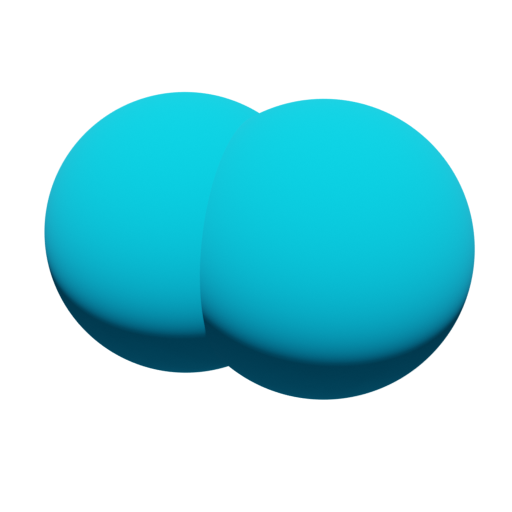
\includegraphics[width=\textwidth]{Images/Union}
		\caption{Union}
	\end{subfigure}
	\hfill
	\begin{subfigure}[t]{0.3\textwidth}
		\centering
		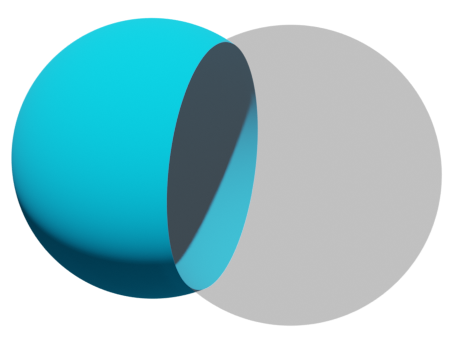
\includegraphics[width=\textwidth]{Images/Difference}
		\caption{Difference}
	\end{subfigure}
	\hfill
	\begin{subfigure}[t]{0.3\textwidth}
		\centering
		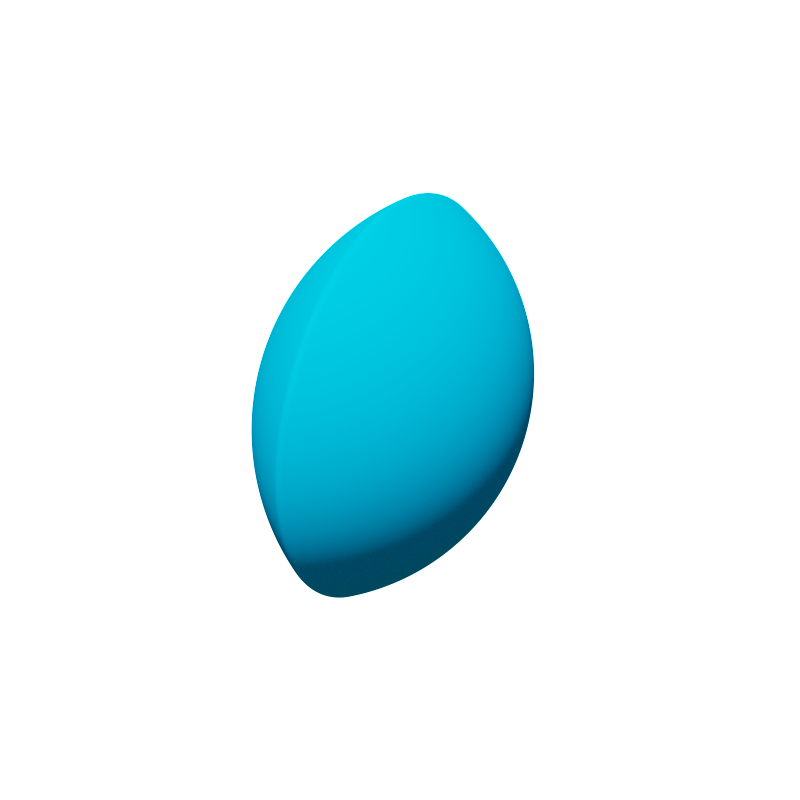
\includegraphics[width=\textwidth]{Images/Intersect}
		\caption{Intersect}
	\end{subfigure}
	\caption{Three boolean operations applied to two spheres: (a) Union operation includes points encompassed by either sphere, (b) Difference operation includes points encompassed by only the first sphere, (c) Intersect operation includes points encompassed by both spheres.}
	\label{fig:boolean operations}
\end{figure}

CSG and other primitive fitting techniques are topics of interest as they resemble Biederman's Recognition-By-Components theory for how humans comprehend 3D shapes. This theory suggests that the human brain decomposes scenes into simple volumes called geons. Biederman theorizes that every brain uses the same set of 36 geon primitives to approximate complex shapes~\cite{Biederman1987}. The theory is supported by the techniques artists use to construct human anatomy. The first step in drawing a figure is to block out the volume using a combination of geometric and organic volumes. These shapes can range from cuboids and cylinders to ellipsoids and pear shapes~\cite{Winslow2015}. Due to their similarity, researchers believe that the Recognition-By-Components theory sets a positive precedent for the use of CSG representations in deep learning~\cite{Sharma2018}.

Instead of using geons, prior work~\cite{Sharma2018, Kania2020, Ren2021} represents CSG primitives as Signed Distance Fields (SDFs). An SDF is a mathematical function that implicitly defines the surface of a volume. Given a query point, an SDF returns the shortest distance from the query point to the represented surface. This distance is positive ($+$) when the query point is outside of the volume and negative ($-$) when the query point is inside. We define the surface as the set of all input points for which the SDF returns 0 (i.e. the zero-level set). The implicit nature of SDFs results in smooth, detailed, and continuous surfaces~\cite{Park2019}. Additionally, SDFs make for good CSG primitives since applying boolean operations to distance fields is trivial.

\begin{figure}
	\centering
	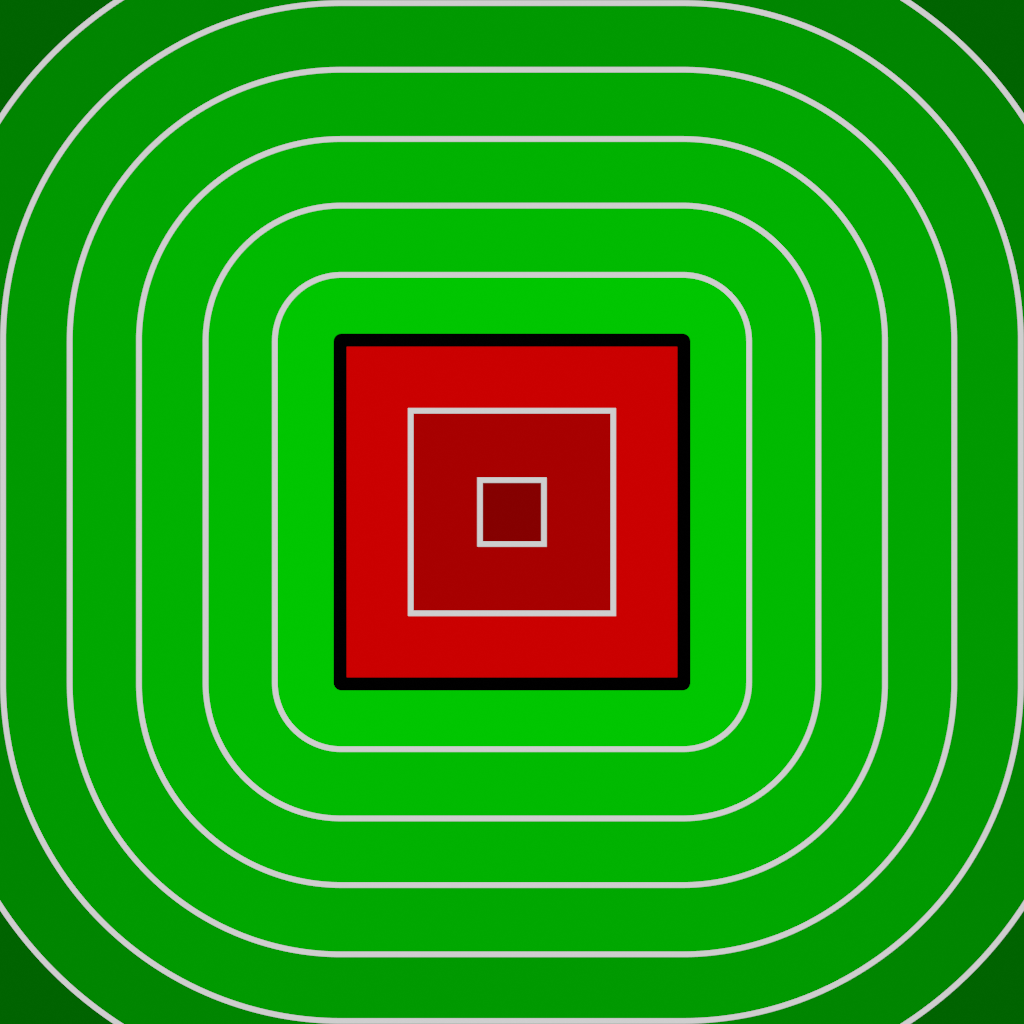
\includegraphics[scale=0.2]{Images/SDF Box}
	\caption{Visualization of the SDF of a 2D box. The surface of the box is depicted in black, the exterior in green, and the interior in red. Points farther from the surface are colored darker. Each of the white contour lines consist of points that are equidistant from the surface.}
	\label{fig:sdf_box}
\end{figure}

There are several benefits to using CSG models for deep 3D reconstruction. The low-dimensionality of a CSG model allows for more efficient training of the network. The continuous and watertight surfaces produced by CSG are visually pleasing. And a key benefit that most other representations lack is an easily modifiable format.

However, there are also several challenges in using a CSG representation. The first issue is the lack of uniqueness~\cite{Hughes2013}. Since there are multiple valid ways to reconstruct a volume using CSG, a network cannot be supervised using expected output samples. The second challenge is that combining geometric primitives directly without applying any blending results in sharp intersections. This is a not an issue when modeling angular mechanical components. Smooth and organic surfaces, on the other hard, cannot be elegantly represented without blending primitives together.

Previous work~\cite{Sharma2018, Kania2020, Ren2021} successfully implements CSG based reconstruction algorithms using unsupervised learning. While succeeding in representing simple geometry, prior work fails to incorporate primitive blending to address the poor reconstruction quality of smooth surfaces. Furthermore, these models only generate a small number of primitives. The CSG-Stump architecture~\cite{Ren2021} supports a maximum output of 256 total primitives in the paper, of which only a subset is selected for use in reconstruction. This number is sufficient to represent simple 3D shapes but fails to capture the details in more complex geometry. Although the architecture can be scaled up, the network complexity, memory requirements, and training time increase non-linearly with the output size~\cite{Ren2021}.

\begin{figure}[!b]
	\centering
	\begin{subfigure}[t]{0.45\textwidth}
		\centering
		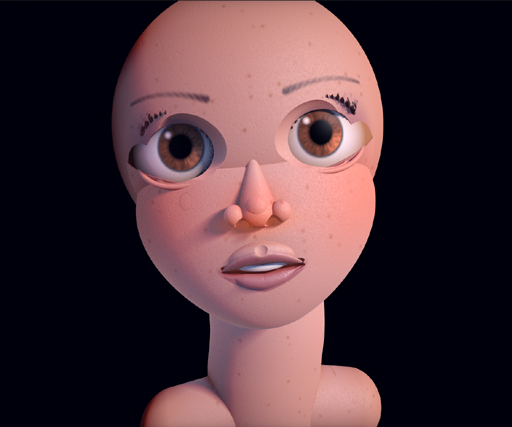
\includegraphics[width=\textwidth]{Images/Face without blending}
		\caption{Without Blending}
	\end{subfigure}
	\hfill
	\begin{subfigure}[t]{0.45\textwidth}
		\centering
		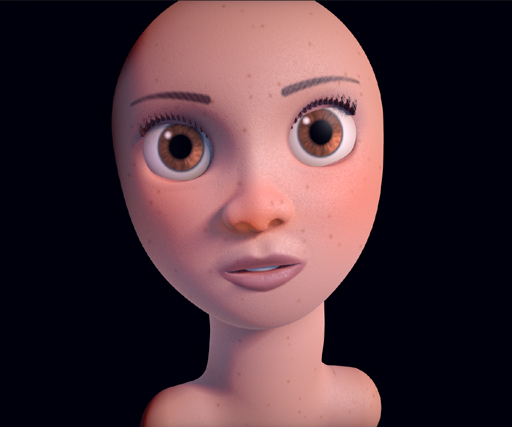
\includegraphics[width=\textwidth]{Images/Face with blending}
		\caption{With Blending}
	\end{subfigure}
	\caption{Demonstration of the importance of primitive blending for modeling organic shapes such as faces using CSG~\cite{Quilez2013}.}
	\label{fig:primitive_blending}
\end{figure}

To address these shortcomings, we propose CSG-CRN: a novel architecture for iteratively generating CSG reconstructions of unlimited size. This is achieved using cascaded refinement, wherein a refinement network recursively improves upon its own output. By iteratively building a reconstruction, our architecture can be kept small while achieving high reconstruction quality. CSG-CRN is an autoencoder network that takes point clouds as input and outputs SDF primitives. The Siamese encoder network generates a feature vector for both the target geometry and the current reconstruction. Then the GRU decoder network analyzes the differences in the feature vectors and generates multiple SDF primitives to refine the reconstruction. The decoder output parameters include a blending factor for each primitive to better represent smooth, organic surfaces. For further refinement, the reconstruction can be fed back into the CSG-CRN network to generate additional primitives. Unlike previous work, the reconstruction time of CSG-CRN scales linearly with the level of detail. To our knowledge, this is the first approach that applies cascaded refinement to the synthesis of CSG models.

We make two main contributions in this work. First, we propose CSG-CRN, a novel architecture for generating CSG reconstructions through cascaded refinement. Second, we conduct experiments to demonstrate the following:

\begin{itemize}
	\item CSG-CRN can efficiently reconstruct a variety of known and unknown shape classes.
	\item CSG-CRN generates qualitatively and quantitatively superior reconstructions than prior CSG-based reconstruction networks.
	\item The CSG-CRN encoder network is capable of inferring missing geometry based on known shape priors.
	\item The CSG-CRN encoder produces a continuous latent space that can be interpolated.
\end{itemize}

\vspace{1em}

The outline of this paper is as follows. The next chapter, \nameref{chap:related_work}, discusses the different 3D representations and neural architectures used by prior work in 3D reconstruction. The \nameref{chap:background} chapter details the mathematics of SDFs and the neural architectures used in the implementation of CSG-CRN. In the \nameref{chap:implementation} chapter, we outline the architecture of CSG-CRN and the methodologies used to train it. The \nameref{chap:experiemnts_and_results} chapter contains the procedures and results for each experiment we conducted. Lastly, the \nameref{chap:conclusion} chapter summarizes our findings in this paper and discusses potential future work.
